%ÁLTALÁNOS KOMMENT: ne taglalad annyira a bekezdéseidet, ha nem muszáj. Lehetőleg egy bekezdés legyen legalább 2 mondat, de inkább több. Ez nem csak ide vonatkozik persze
\chapter{Felhasználói dokumentáció}
\label{ch:user}

Az általam fejlesztett szoftver két felhasználói felülettel rendelkezik.
Az egyik egy parancssoros (CLI) program az adathalmaz generálásához,
a másik egy grafikus (GUI) alkalmazás az átalakítások szemléltetéséhez,
és az adathalmaz böngészéséhez.
Mindkét alkalmazás felületének nyelve angol.

\section{Futtatási környezet}

A szoftver egy Python 3.10-es vagy újabb verziójú Python értelmezővel futtatható.
Futtatás előtt a szoftver függőségeit installálni kell a \emph{pip} csomagkezelővel.
Ezt a legegyszerűbben a szoftver forráskódjának könyvtárából tehetjük meg,
a következő parancs kiadásával:

\begin{lstlisting}[language=bash, numbers=none]
	$ pip install --editable .
\end{lstlisting}

\section{Adatbázis beállítása}

Az adathalmaz generálásához szükség van egy \emph{mongodb} adatbázis kliensre \cite{installMongodb}.
Az adatbázis kiszűri a kódpárok generálása közben a duplikált kódokat,
és az adatok lekérdezését is megkönnyíti.

Az adatbázis elérését a forrás könyvtárában a \emph{config/default.ini} útvonal alatt található
konfigfájlban lehet beállítani.
Egy adatbázist három paraméter határoz meg: \emph{host}, \emph{port}, \emph{database} (az adatbázis neve).
Ha szükséges a konfigfájl alapértékeit átírhatjuk.

\section{Adathalmazt generáló CLI}

A szoftver CLI alkalmazásával van lehetőségünk az adathalmaz generálására egy
adott csv fájlban található kódokból vagy egy könyvtárban taláható forrásfájlokból.
Adathalmazt a következő paranccsal generálhatunk:

\begin{lstlisting}[language=bash, numbers=none]
	$ python -m source.persistor <mode> <path>
\end{lstlisting}

A parancs paraméterei a következők:

\begin{enumerate}
	\item\label{step:first} \emph{mode} - az adatok forrásának típusa,
	lehetséges értékek:
	\begin{itemize}
		\item \emph{csv} - csv fájlból olvassa a forrásfájlok tartalmát
		\item \emph{dir} - könyvtárból rekurzívan olvassa a forrásfájlokat
	\end{itemize}
	\item \emph{path} - az adatok forrásának elérési útvonala
\end{enumerate}

Ha megadtuk a \lstinline{peristor} parancsot, a program megpróbálja a forráskódok olvasását,
ha az input nem megfelelő, akkor leáll.
Futtatás közben a program kiírja az éppen feldolgozott forráskóddal kapcsolatos információkat,
például a kódon végzett átalakítások számát, és azt, hogy el tudta-e menteni az átalakítások eredményeit.

\begin{figure}[H]
	\centering
	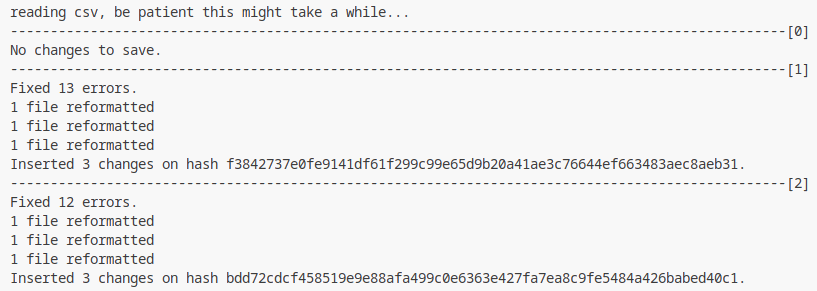
\includegraphics[width=0.9\textwidth,frame]{images/screenshots/log.png}
	\caption{A CLI alkalmazás futás közben}
\end{figure}

Ha a program végigolvasta a csv fájlt vagy a könyvtárban található forrásfájlokat, leáll.
Amikor a program megállt, a forráskód-párok már az adatbázisban vannak,
a \emph{mongoexport} eszköz segítségével az adatbázisból a forráskód-párokat
egy csv fájlba exportálhatjuk.

\section{Átalakításokat szemléltető GUI}

A szoftver GUI alkamazása szemlélteti az átalakításokat.
Kipróbálhatunk vele egy vagy több átalakító szabályt,
vizualizálhatjuk kódok absztrakt szintaxisfáját,
és az adatbázisba bekerült átalakítások eredményét is megnézhetjük.

\subsection{Alkalmazás indítása}

Az alkalmazás a forrás könyvtárából indítható a következő paranccsal:

\begin{lstlisting}[language=bash, numbers=none]
	$ python -m source
\end{lstlisting}

A parancs kiadása után a felugró ablakban beállíhatjuk az adatbázis kapcsolathoz szükséges paramétereket:
a \emph{host}, \emph{port} illetve \emph{database} értékeit (lásd \ref{fig:launcher}. ábra).
A \emph{Connect} gombra kattintva az alkalmazás adatbáziseléréssel indul,
ha a megadott adatbázishoz 10 másodperc alatt kapcsolódni tud,
különben adatbáziselérés nélkül fog elindulni.
Adatbáziselérés nélkül a \emph{Launch Now} gombbal indíthatjuk az alkalmazást.

\begin{figure}[H]
	\centering
	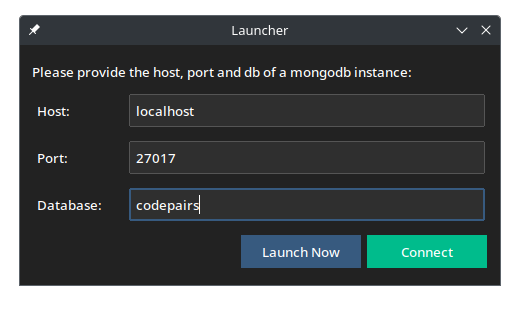
\includegraphics[width=0.5\textwidth]{images/screenshots/launcher.png}
	\caption{\label{fig:launcher}Az alkalmazást indító ablak}
\end{figure}

\subsection{Alkalmazás felülete}

Az GUI alkalmazás felülete funkciók szerint két fő nézetre osztható, a refaktoráló és az adatbázis-böngésző nézetre.
A menü gombjai és az állapotsor szövegei a két fő nézeten kívül helyezkednek el.

A refaktoráló nézetben (\emph{Refactor} tab) egy kódon
ekvivalensen és nem ekvivalensen átalakító szabályokat próbálhatunk ki, és elmenthetjük
a szabályok által végzett átalakítások eredményeit.
Az adatbázis-böngésző (\emph{Database} tab) nézetben az adatbázisba bekerült kódpárokat tekinthetjük meg.

\subsection{Refaktoráló nézet}

Indítás után a felhasználót a refaktoráló nézet fogadja.
Egy Python forráskód átalakításához a kódot begépelhetjük a \emph{Source Code} szöveges input mezőbe,
vagy egy \emph{.py} kiterjesztésű fájlból is betölthetjük a menüben látható \emph{Open File} gombra kattintva.

\begin{figure}[H]
	\centering
	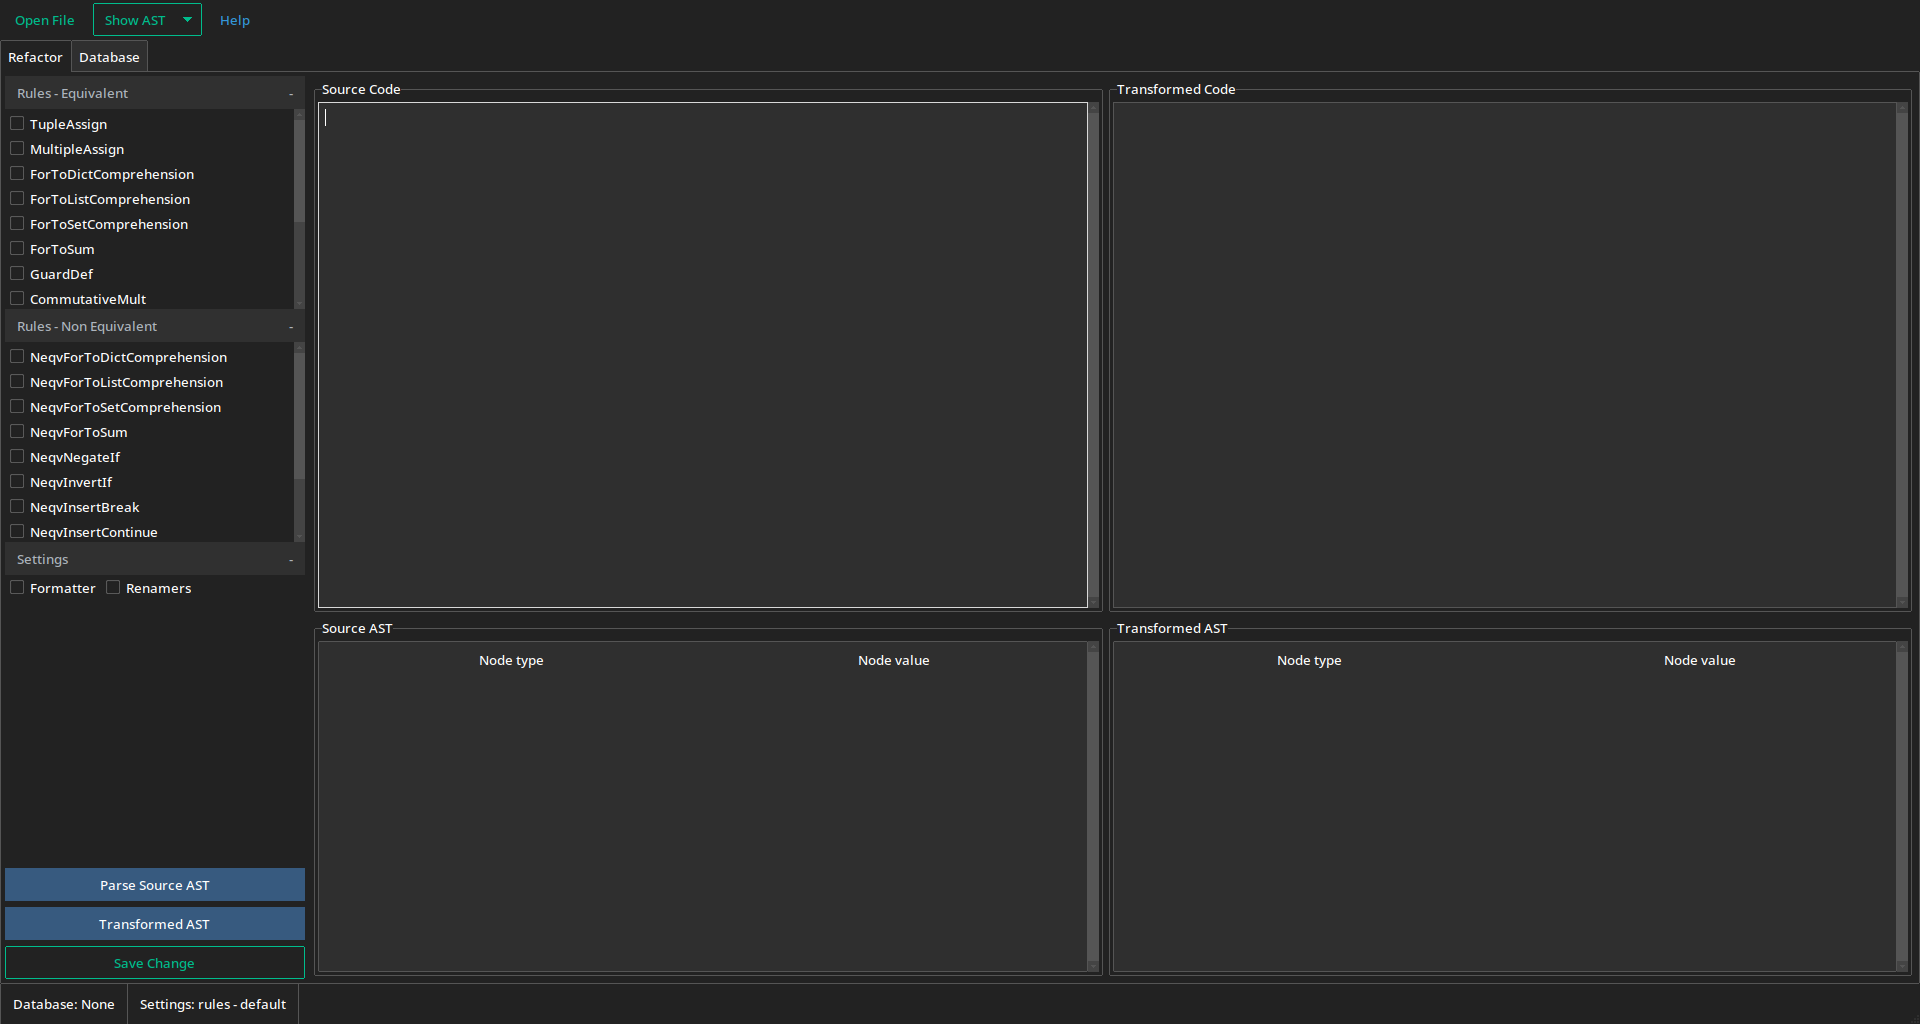
\includegraphics[width=0.9\textwidth]{images/screenshots/refactor_tab_1.png}
	\caption{Refaktoráló nézet az indítás után}
\end{figure}

Az átalakítás előtt a begépelt vagy betöltött forráskódból létre kell hozni egy AST-t
az elemező (parser) futtatásával,
ezt a \emph{Parse Source AST} gombbal tehetjük meg. Ha a megadott forráskódban szintaxis hiba található, 
vagy valami egyéb okból kifolyólag nem elemezhető, akkor az alkalmazás ezt jelzi egy felugró 
párbeszéd-ablakkal. Akkor is jelez, ha parse-olás nélkül klikkelünk az átalakító gombra.

\begin{figure}[H]
	\centering
	\subcaptionbox{elemzési hiba esetén}{
		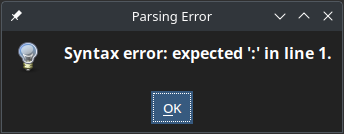
\includegraphics[width=0.5\linewidth]{images/screenshots/syntax_error.png}}
	\hspace{5pt}
	\subcaptionbox{hiányzó AST esetén}{
		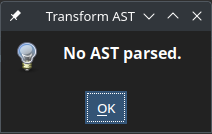
\includegraphics[width=0.31\linewidth]{images/screenshots/no_ast_parsed.png}}
	\caption{Hibákat jelző párbeszéd-ablakok}
\end{figure}

Sikeres elemzés után az AST felépítését a \emph{Source AST} fa nézeten láthatjuk, 
az első oszlopban a csúcs típusa, a második oszlopban a csúcs szintaxisfájából
generált kód látható. 

Elemzés után a fát átalakíthatjuk a \emph{Transform AST} gombra kattintva, 
ekkor az átalakított fa megjelenik a bal oldali \emph{Transformed AST} fa nézeten,
az átalakított fából generált kód pedig a \emph{Transformed Code} readonly szövegdobozban.

\begin{figure}[H]
	\centering
	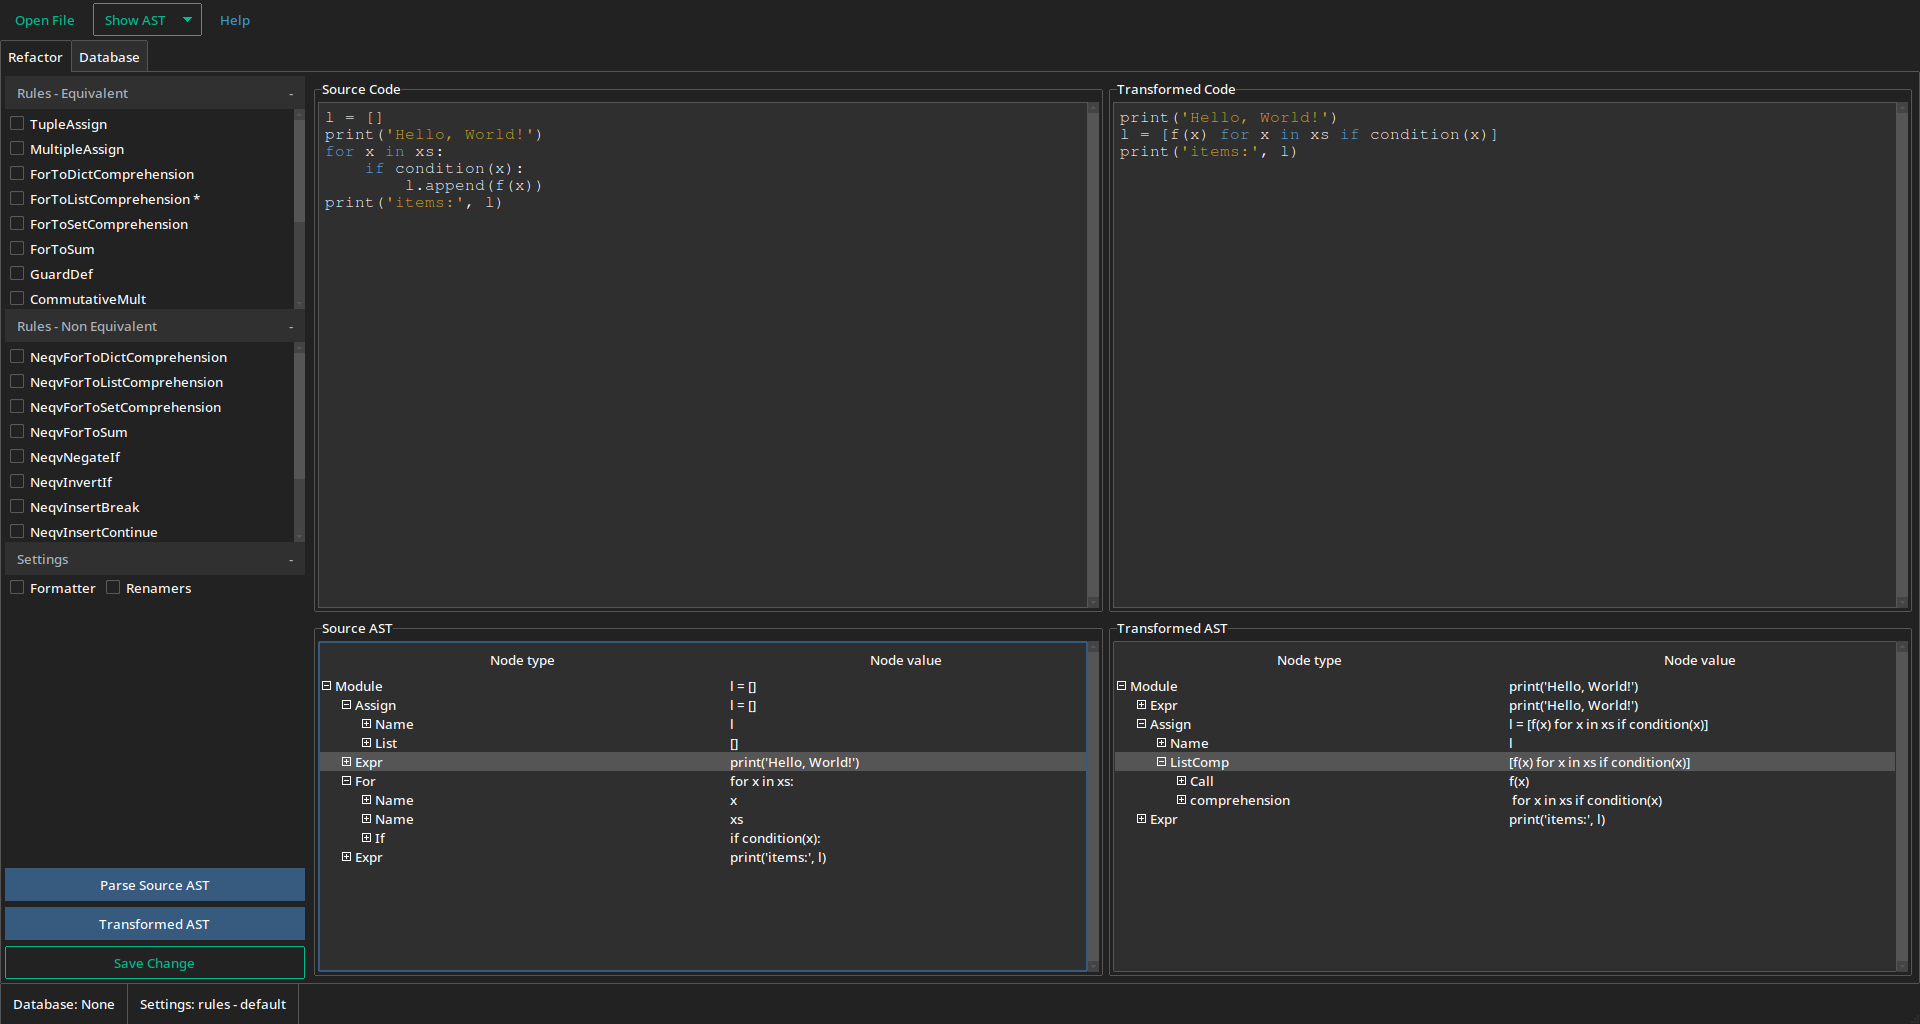
\includegraphics[width=0.9\textwidth]{images/screenshots/refactor_tab_2.png}
	\caption{Példa egy átalakítás eredményére}
\end{figure}

Az alkalmazás összesen 28 átalakító szabályt használ, ezek közül 16 ekvivalens és 12 nem ekvivalens
eredményt állít elő.
Az alkalmazás indításakor az összes ekvivalens szabály ki van választva,
ez az alkalmazás alapbeállítása, amit a \emph{'rules - default'} felirat jelez az állapotsorban.

Lehetőségünk van általunk választott szabályok alkalmazására is.
A szabályok listája a bal oldali panelen látható. Minden szabály előtt van egy checkbox
amivel a szabályt kiválaszthatjuk. Lehetőségünk van egy vagy több szabály kiválasztására is,
így könnyen tesztelhetjük egy szabály működését.
Ha vannak kiválasztott szabályok, azt a \emph{'rules - custom'} felirat jelzi az állapotsorban.

Átalakításkor a szabályok a bal oldali panelen látható sorrendben, fentről lefele kerülnek végrehajtásra.
A panelen a szabályokon kívül található még két checkbox is,
ezekkel a \emph{ruff} formatter és az átnevező átalakítások alkalmazását tudjuk beállítani.

Miután átalakítottunk egy forráskódot, kimenthetjük az átalakítás eredményét az adatbázisba,
ha van adatbázis kapcsolat.
Ezt a refaktoráló nézet bal alsó sarkában elhelyezkedő \emph{'Save Change'} gombra kattintva
tehetjük meg.
Ha az átalakítást adatbázis kapcsolat hiánya miatt nem lehet elmenteni,
akkor azt az alkalmazás párbeszéd-ablakban jelzi.

\subsection{AST-k vizualizálása}

Az alkalmazással vizualizálhatjuk az általunk megadott vagy az átalakított kód AST-jét.
Az AST-k ábráit a \emph{Show AST} lenyíló menügombbal készíthetjük el, a gombra klikkelve két opció közül választhatunk:
a \emph{Source} az általunk megadott kód, a \emph{Transformed} az átalakított kód AST-jét vizualizálja.
Az alkalmazás jelzi ha a kiválasztott AST még nem jött létre, különben elkészíti az AST ábráját.
A kész ábrát egy felugró ablakban nyitja meg.
A \ref{fig:ast_example}. ábra például az alkalmazással készült, az ábrán a \emph{helloworld} Python kódjának AST-je szerepel:

\begin{figure}[H]
	\centering
	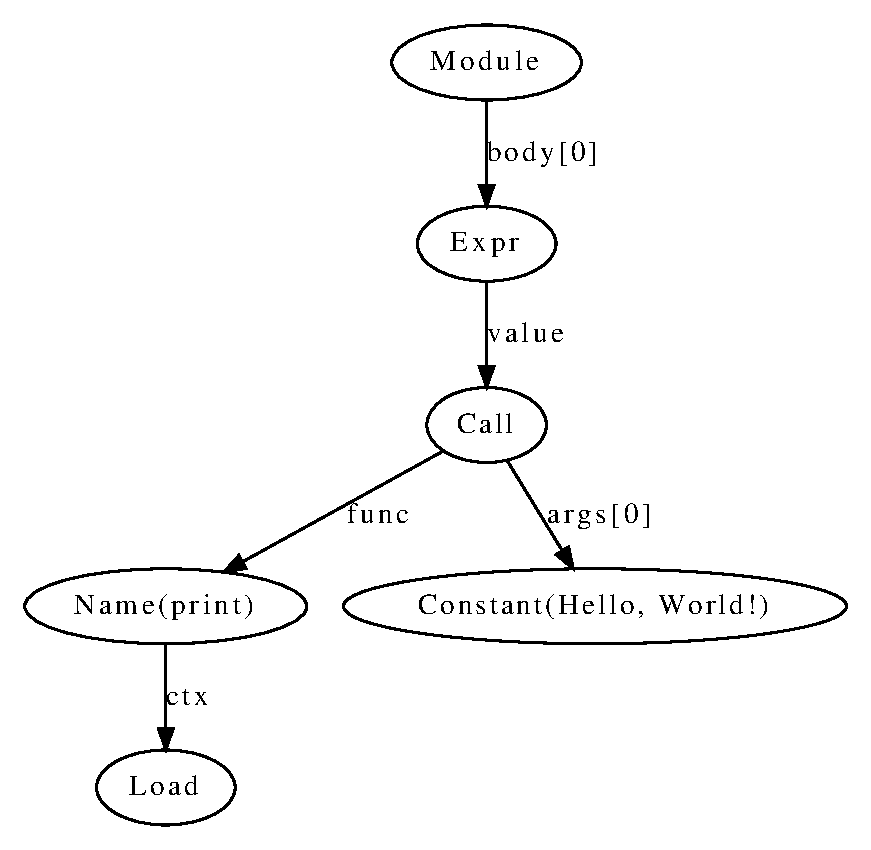
\includegraphics[width=0.6\textwidth]{images/figs/ast_graph.eps}
	\caption{\label{fig:ast_example}A \emph{helloworld} program AST-je}
\end{figure}

\subsection{Adatbázis-böngésző nézet}

Ebben a nézetben megtekinthetjük az adatbázisba bekerült forráskód-párokat.
A nézet csak akkor jön létre, ha az alkalmazásnak van adatbázis elérése,
ha nincs, azt a nézeten a \emph{"No database connection."} felirat jelzi.
A nézet feladata a forráskód-párok listázása, és a párba állított forráskódok
különbségeinek megjelenítése.

A különbségeket két forráskód között könnyen vizualizálhatjuk egy diffel,
azaz olyan szövegösszehasonlító programmal, ami a szövegek közti a különbségek
listáját állítja elő.
A különbségeket a forráskód-párokban ezzel a módszerrel vizualizálom.

\begin{figure}[H]
	\centering
	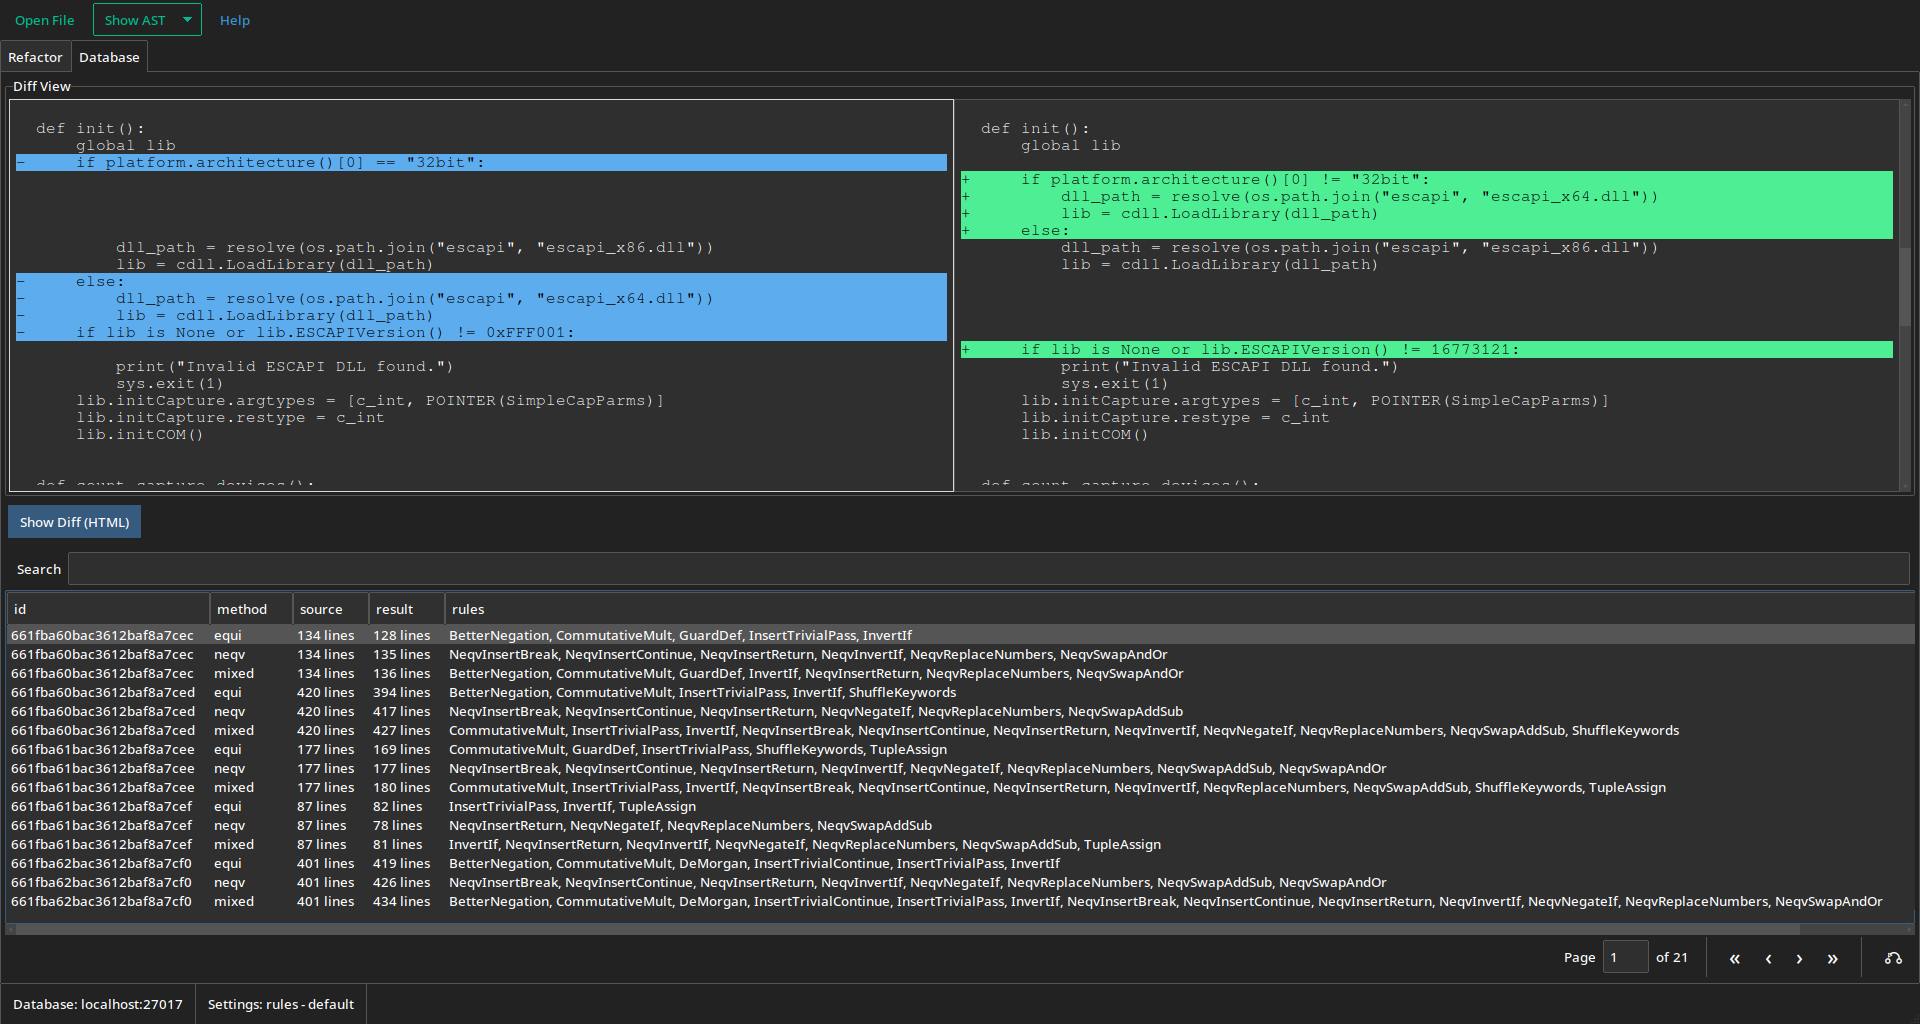
\includegraphics[width=0.9\textwidth]{images/screenshots/database_tab.png}
	\caption{Adatbázis-böngésző nézet}
\end{figure}

A nézet tetején találhatóak a diffeket megjelenítő szövegdobozok, ezek alatt
egy táblázat látható, soraiban az adatbázisba bekerült forráskód-párokkal.
A táblázat soraiban található adatok sémáját a \ref{tab:schema}. táblázat írja le.

\begin{table}[H]
	\centering
	\begin{tabular}{ | m{0.15\textwidth} | m{0.75\textwidth} | }
		\hline
		\textbf{Oszlop} & \textbf{Magyarázat} \\
		\hline \hline

		\emph{id}
		& az eredeti forrráskód azonosítóját tartalmazó oszlop \\
		\hline
		
		\emph{method}
		& az átalakításra használt módszerre utaló oszlop
		
		(például a szabályhalmazra) \\
		\hline
		
		\emph{source}
		& az eredeti forráskód sorainak számát tartalmazó oszlop \\
		\hline
		
		\emph{result}
		& az átalakított forráskód sorainak számát tartalmazó oszlop \\
		\hline
		
		\emph{rules}
		& az átalakításnál alkalmazott szabályok listája (szöveg) \\
		\hline
	\end{tabular}
	\caption{Adatbázis-böngésző nézet táblázatának oszlopai}
	\label{tab:schema}
\end{table}

Ha a táblázat egy sorára, vagyis egy forráskód-párra
%tippre nem kell kötőjel (akkor kell tudtommal, ha legalább 6 szótag és 3 szó az összetett szó. De nem tudom azóta ez a szabály hogy van...) szóval DIKK (idk (hehe))
klikkelünk,
akkor a diff nézetben megjelennek az eredeti (bal oldali) és az átakított (jobb oldali)
kód közti különbségek.

A forráskód-párok böngészéséhez a táblázat feletti keresőt használathatjuk.
A kereső az összes sorban és oszlopban szereplő adatok közt keres.
Például megkereshetjük, hogy az adatbázisban mely forráskódokon kerültek alkalmazásra
for ciklussal kapcsolatos átalakítások.
